\section{Roadmap}\label{roadmap}

% Describe the system and its connection with concepts mentioned before. Everything bellow is new!

The system developed in this research is inspired by the concepts of interactive music systems and intended for the average user.
It sees both silent disco and flash mobs as significant conceptional roots.
Whereas silent disco will be referred as a context for the system existent, flash mobs are associated as a social phenomena that use new technologies to facilitate creative, or even artistic social behavior, with emphasis on social interaction.

From the participants point of view the system will consist of few balloon bundles, each one corresponds to a specific musical style.
When the participants will stroll between the balloon bundles with their mobile devices and headphones their relative distances from the different bundles will affect the music in their headphones, creating virtual ``sound zones'' around each balloon bundle.
The distance between each participant and sound zones may affect the music in several different ways.
For example, when a participant get close to specific sound zone the music filtration may change according to the distance.
For another sound zone the volume may be changed when getting close to it or walk away.
Although the style of each sound zone will be well-definition, every sound zone will by able to be heard with any other sound zone, in synchronization and harmony.
In addition, participants will be able to freely move the balloon bundles, thereby changing the structure of the music in the virtual space\footnote{A video demonstrating the system behavior from the participant point of view can be found at \href{http://youtu.be/2kJoeD2iWBA}{youtu.be/2kJoeD2iWBA}.}.

\begin{figure}[h]
	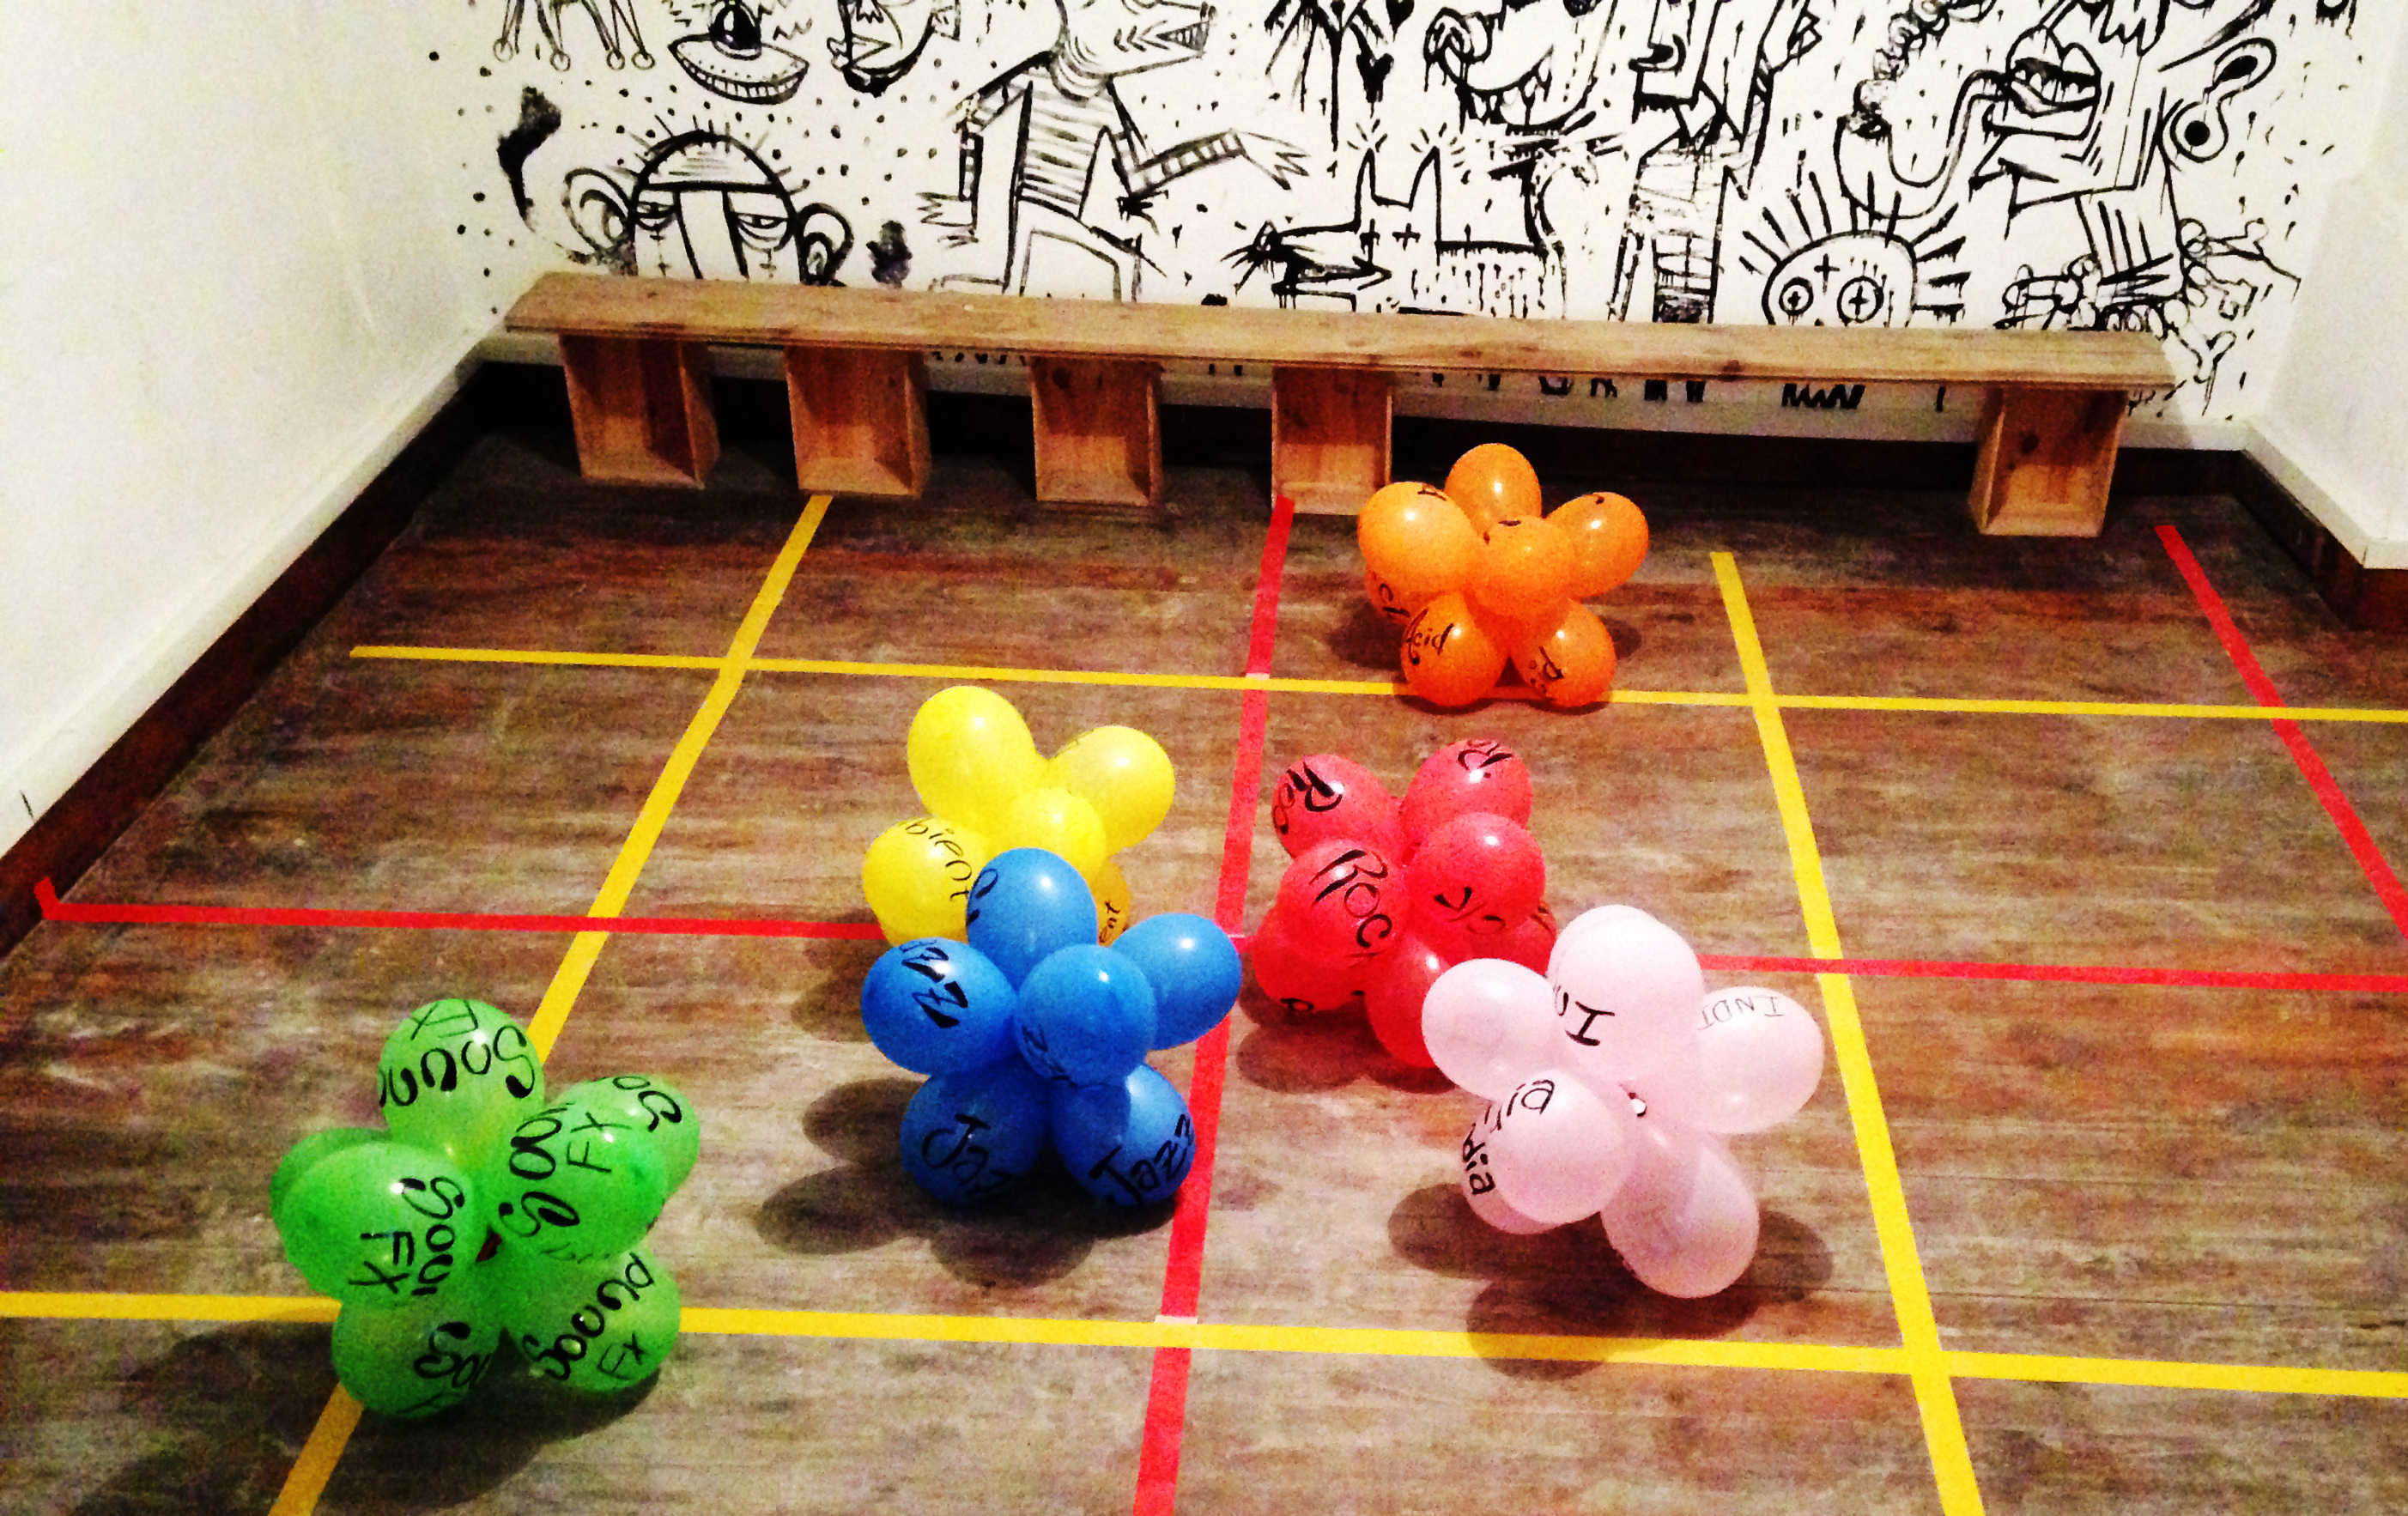
\includegraphics[width=\linewidth]{balloons}
	\caption{Balloon bundles on the dance floor}
\end{figure}

In order to evaluate the social effect of this system I will try to answer the research question: \emph{\reserchquestion}